%%%%%%%%%%%%%%%%%%%%%%%%%%%%%%%%%%%%%%%%%
% Short Sectioned Assignment
% LaTeX Template
% Version 1.0 (5/5/12)
%
% This template has been downloaded from:
% http://www.LaTeXTemplates.com
%
% Original author:
% Frits Wenneker (http://www.howtotex.com)
%
% License:
% CC BY-NC-SA 3.0 (http://creativecommons.org/licenses/by-nc-sa/3.0/)
%
%%%%%%%%%%%%%%%%%%%%%%%%%%%%%%%%%%%%%%%%%

%----------------------------------------------------------------------------------------
%	PACKAGES AND OTHER DOCUMENT CONFIGURATIONS
%----------------------------------------------------------------------------------------

\documentclass[paper=a4, fontsize=11pt]{scrartcl} % A4 paper and 11pt font size

\usepackage[T1]{fontenc} % Use 8-bit encoding that has 256 glyphs
\usepackage{fourier} % Use the Adobe Utopia font for the document - comment this line to return to the LaTeX default
\usepackage[english]{babel} % English language/hyphenation
\usepackage{amsmath,amsfonts,amsthm} % Math packages

\usepackage{lipsum} % Used for inserting dummy 'Lorem ipsum' text into the template

\usepackage{sectsty} % Allows customizing section commands
\allsectionsfont{\centering \normalfont\scshape} % Make all sections centered, the default font and small caps


\usepackage{IEEEtrantools}
\usepackage{listings}
\usepackage{caption}
\usepackage{subcaption}
\usepackage{subfig}
\usepackage{amsmath,amssymb,amsthm}
\usepackage{graphicx}

% Python style for highlighting
\newcommand\pythonstyle{\lstset{
language=Python,
basicstyle=\ttm,
otherkeywords={self},             % Add keywords here
keywordstyle=\ttb\color{deepblue},
emph={MyClass,__init__},          % Custom highlighting
emphstyle=\ttb\color{deepred},    % Custom highlighting style
stringstyle=\color{deepgreen},
frame=tb,                         % Any extra options here
showstringspaces=false            % 
}}


% Python environment
\lstnewenvironment{python}[1][]
{
\pythonstyle
\lstset{#1}
}
{}


\usepackage{fancyhdr} % Custom headers and footers
\pagestyle{fancyplain} % Makes all pages in the document conform to the custom headers and footers
\fancyhead{} % No page header - if you want one, create it in the same way as the footers below
\fancyfoot[L]{} % Empty left footer
\fancyfoot[C]{} % Empty center footer
\fancyfoot[R]{\thepage} % Page numbering for right footer
\renewcommand{\headrulewidth}{0pt} % Remove header underlines
\renewcommand{\footrulewidth}{0pt} % Remove footer underlines
\setlength{\headheight}{13.6pt} % Customize the height of the header

\numberwithin{equation}{section} % Number equations within sections (i.e. 1.1, 1.2, 2.1, 2.2 instead of 1, 2, 3, 4)
\numberwithin{figure}{section} % Number figures within sections (i.e. 1.1, 1.2, 2.1, 2.2 instead of 1, 2, 3, 4)
\numberwithin{table}{section} % Number tables within sections (i.e. 1.1, 1.2, 2.1, 2.2 instead of 1, 2, 3, 4)

\setlength\parindent{0pt} % Removes all indentation from paragraphs - comment this line for an assignment with lots of text

%----------------------------------------------------------------------------------------
%	TITLE SECTION
%----------------------------------------------------------------------------------------

\newcommand{\horrule}[1]{\rule{\linewidth}{#1}} % Create horizontal rule command with 1 argument of height

\title{	
\normalfont \normalsize 
\textsc{Department of Electrical Engineering, IIT Madras} \\ [25pt] % Your university, school and/or department name(s)
\horrule{0.5pt} \\[0.4cm] % Thin top horizontal rule
\huge Assignment 1 - Polynomial Interpolation \\ % The assignment title
\horrule{2pt} \\[0.5cm] % Thick bottom horizontal rule
}

\author{Surajkumar H - EE11B075} % Your name

\date{\normalsize\today} % Today's date or a custom date

\begin{document}

\maketitle % Print the title

%----------------------------------------------------------------------------------------
%	PROBLEM 1
%----------------------------------------------------------------------------------------

\section{Question 1: 5-point 4th order Interpolation}


In this question, we sample the function $f(x)=sin(x+x^2)$ uniformly at 5 points in $[0,1]$. We then use these 5 sample values to interpolate (and extrapolate) the function values at points in the range given by 
\begin{lstlisting}
xx=np.linspace(0,1,5);
\end{lstlisting}

\subsection{Background and Functions}

We examine how polynomial interpolation performs at these values and compare it with the theoretical (known) value of the function at these points. Since we have exactly 5 samples, we run $4^{th}$ order polynomial interpolation on all points in the range. We use the modified Neville's Algorithm. The original algorithm constructs the Lagrangian polynomial recursively, running interpolation on smaller sets (of say $m$) points, and uses adjacent sets to estimate the value of the interpolation using $m+1$ points. The recursive relation is
\begin{equation}
P_{i(i+1)\ldots(i+m)} = \frac{(x-x_{i+m})P_{i(i+1)\ldots(i+m-1)}+(x_{i}-x)P_{(i+1)(i+2)\ldots(i+m)}}{x_i - x_{i+m}}
\end{equation}

where $x$ is the point where the function value is to be inter(extra)polated. By design, the function values coincide with the data values at the known sample points.  

The modified version of the algorithm (which we use here) starts with an initial estimate of the function value (we do this by finding the sample closest to the point of interest), and recursively computing \textit{small differences} between adjacent estimates (using the smaller sets as above). We choose one of these differences at each stage, and add it to the function estimate at the point of interest. Mathematically, we define for $m=1,2,\ldots,N-1$
\begin{IEEEeqnarray}{rCl}
C_{m,i} &=& P_{i(i+1)\ldots(i+m)} - P_{i(i+1)\ldots(i+m-1)} \nonumber \\
D_{m,i} &=& P_{i(i+1)\ldots(i+m)} - P_{(i+1)(i+2)\ldots(i+m)}
\end{IEEEeqnarray}
that is, the upper and lower differences in the ancestor tree (as seen in \cite{NR}). From this, we get

\begin{IEEEeqnarray}{rCl}
C_{m+1,i} &=& \frac{(x_{i+m+1}-x)(C_{m,i+1}-D_{m,i})}{x_{i}-x_{i+m+1}} \nonumber \\
D_{m+1,i} &=& \frac{(x_{i}-x)(C_{m,i+1}-D_{m,i})}{x_{i}-x_{i+m+1}} \label{nev1}
\end{IEEEeqnarray}

At each level $m$, the $Cs$ and $Ds$ represent the corrections made to the value estimate. We recursively compute these corrections using \ref{nev1}. We then choose a path through the ancestor tree which connects the final interpolated value ($m=N-1$), to the initial estimate. We then add all these corrections to get the interpolated value at the point $x$. In our implementation of the algorithm, we chose the correction based on whether the index estimate is above / below the average ($\frac{N-m}{2}$). This way, we ensure  movement towards the rightmost element correctly. 

A general python function \textsc{polint} was written, which computes the $N^{th}$ order interpolated value at a single point from the set of data points and values. The function \textsc{findnearest} takes an input point, the entire data set, the order of interpolation $N$, and computes indices of the nearest $N$ data points. Later, we test how the error varies with the order of interpolation. It is very helpful to have a function which finds the closes $N$ samples for a given value, since we can use these to interpolate the function value at the unknown point $x$. Finally, we used $\textsc{nearestpolint}$ to perform point by point inter(extra)polation on every point in $xx$ (set of unknown values). 

\begin{figure*}
        \centering
        \begin{subfigure}{.5\textwidth}
  \centering
        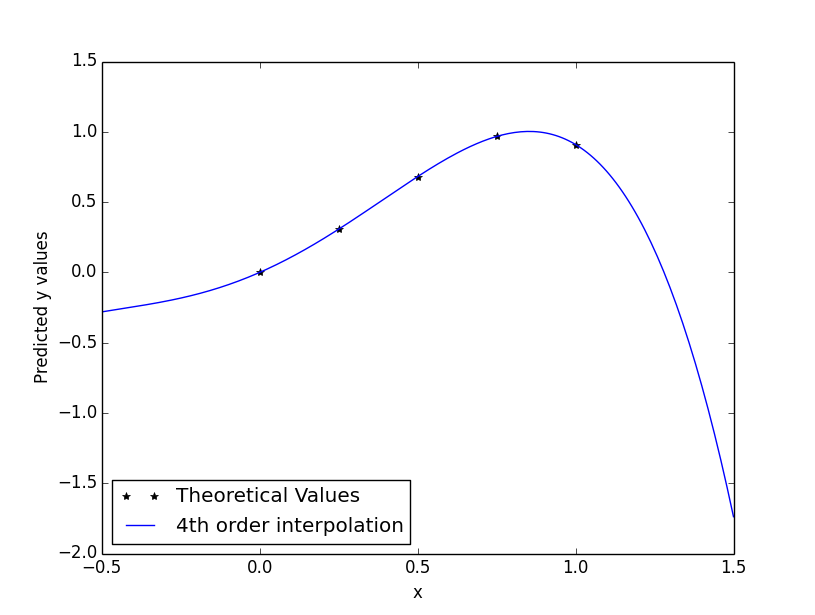
\includegraphics[width=\linewidth]{q1/interpol.png}
                \caption{Theoretical and interpolated values of $f(x)$}
                \label{fig:q1_inter}
                \end{subfigure}%
\begin{subfigure}{.5\textwidth}
  \centering
        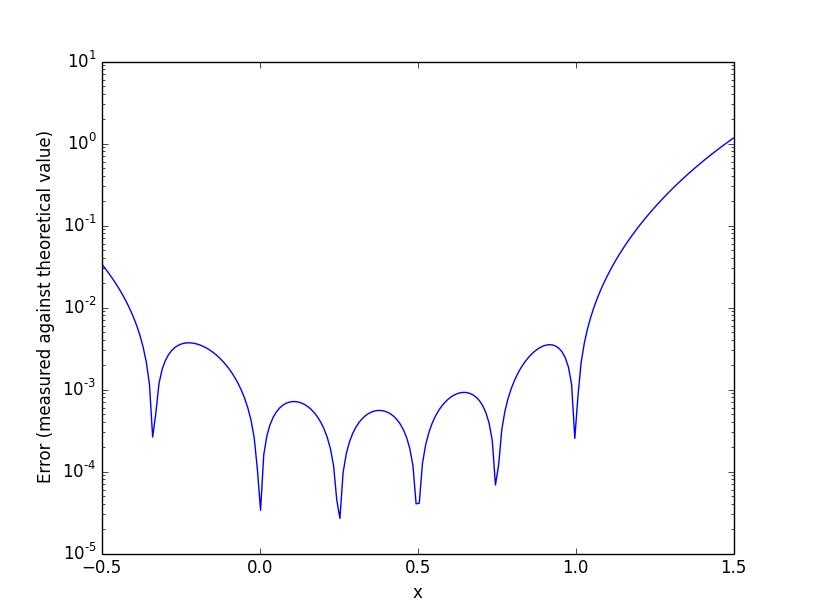
\includegraphics[width=\linewidth]{q1/error_log.png}
                \caption{$4^{th}$ order Interpolation error}
                \label{fig:q1_error}
	\end{subfigure}
            
\caption{Comparison of theoretical and $4^{th}$-order inter(extra)polated function values, and the absolute error in interpolation}
\label{fig:q1}            
\end{figure*}

\subsection{Interpolation, Extrapolation and Error}

Figure (\ref{fig:q1_inter}) shows the comparison of the theoretical, and the 4th order interpolated value at the intermediate and outer points. Figure (\ref{fig:q1_error}) shows the error in 4th order interpolation, taken with respect to the theoretical function values at the point (given by $f(x)$). We clearly see that the error at the interpolated points is of the order $10^{-3}$ for middle points, and $~10^{-2}$ as we move closer to the edge. This makes sense, as the data at the edge doesn't give us equal information on how the function behaves on both sides (which middling values give us). The spike values indicate the known points, where the error is $0$ (the log should be $-\infty$, but python ignores the value), and the points very close to the known point have a smaller error. As we go closer to the midpoint between any 2 known values, the error increases. 

The behaviour beyond $[0,1)$ is a lot more unpredictable. For this particular function, the error increases as we move further away from the known points. We are using $N^{th}$ order (N=4) interpolation. We are trying to fit an $Nth$ order polynomial to a given set of $N$ points. As we can clearly see the polynomial fit $\to\pm\infty$ as $x\to\pm\infty$. This means as we go further away from the known data points, the extrapolated function blows up. Since the actual $f(x)$ is bounded (maximum value is $1$), the error value grows larger with $x$ (cannot guarantee monotonicity).

\section{Question 2: 30-point 4th order Interpolation} 

\begin{figure*}
        \centering
        \begin{subfigure}{.5\textwidth}
  \centering
        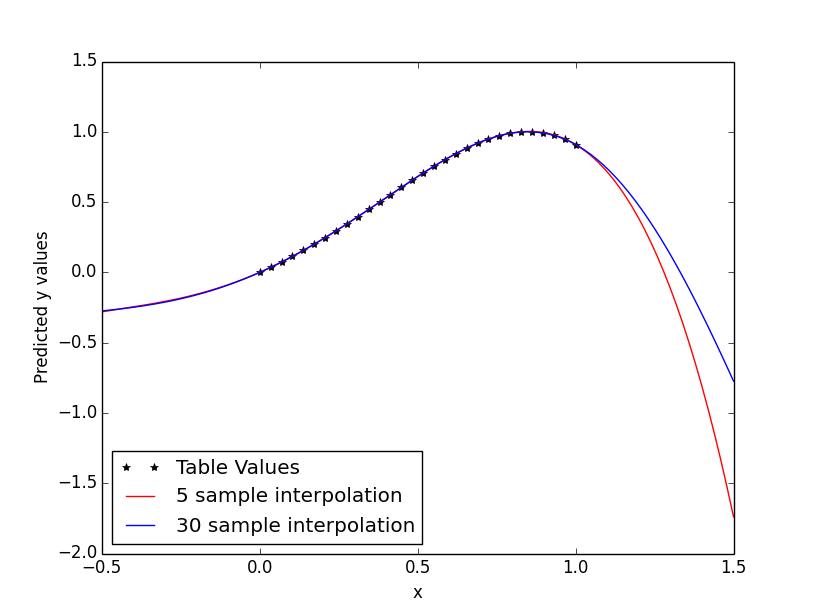
\includegraphics[width=\linewidth]{q2/interpol.png}
                \caption{Theoretical and interpolated values of $f(x)$}
                \label{fig:q2_inter}
                \end{subfigure}%
\begin{subfigure}{.5\textwidth}
  \centering
        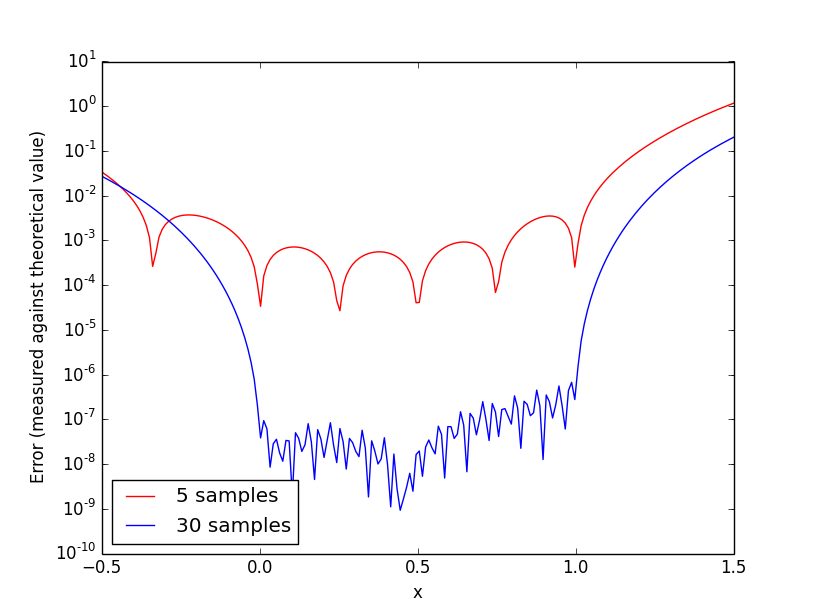
\includegraphics[width=\linewidth]{q2/error_log.png}
                \caption{Comparison of $4^{th}$ order Interpolation error run for 5 and 30 sample points}
                \label{fig:q2_error}
	\end{subfigure}
            
\caption{Comparison of theoretical and $4^{th}$-order inter(extra)polated function values obtained using 5 and 30 sample points}
\label{fig:q2}            
\end{figure*}

In this problem, we investigate the effect of higher sample point density on interpolation. Specifically, we compare the previous case of $4th$ order interpolation with 5 sample points, to $4th$ order interpolation with 30 sample points. We use \textsc{findnearest} to find the nearest 5 points for any given point, and then use \textsc{polint} to find thee interpolated value. We run this over the same data set as in the first question. 

Intuitively, we expect denser interpolation to give much lower error. This is because we fit the same order polynomial over a much closer set of points. Since the function is 'nice' (the function doesn't have discontinuous derivatives), the local behaviour of the function described by 5 close sample points should give a closer approximation of the function, as compared to 5 far away points. 

Figure (\ref{fig:q2_inter}) shows the comparison of the theoretical, the 5 sample and the 30 sample interpolation. Figure (\ref{fig:q2_error}) shows the absolute error comparison for the 2 cases. The plot agrees with our intuition. The interpolation error is roughly $~10^{-3}$ for the 5 sample version, and $~10^{-7}$ for the 30 sample version.

\begin{thebibliography}{155}
\bibitem{NR}
William H. Press, Saul A. Teukolsky, William T. Vetterling, Brian P. Flannery, "Numerical Recipes in C" 

\bibitem{Stoer}
J. Stoer, R. Bulirsch, "Introduction to Numerical Analysis"

\end{thebibliography}

\end{document}